\documentclass[12pt]{article}

\usepackage{times}
\usepackage{graphicx}
\usepackage[letterpaper, width=6in, top=1.25in, bottom=1.25in]{geometry}
\usepackage{nopageno}
\usepackage[justification=raggedright, singlelinecheck=false, labelfont=bf, skip=0pt]{caption}

\begin{document}

\section*{Micron CellularRAM Burst Memory Controller}

\section{Summary}

This design provides a burst-mode synchronous interface to the Micron 16 MB (8M $\times$ 16) pseudo-SRAM chip commonly found on Digilent Nexys-2 and Nexys-3 FPGA development boards. Default settings are for 32-word burst length and 7-clock latency (to allow internal refresh cycles at the start of read or write bursts).  At the maximum clock frequency of 80 MHz, the net transfer rate is approximately 120 MB/sec.

\vspace{\baselineskip}
\noindent
\includegraphics[width=6in]{block_diagram.pdf}


\section{Interface}

On FPGA startup the RAM is reconfigured to allow synchronous burst access; once this is completed, and after completion of each data transfer, \texttt{ready} is asserted high to indicate that a new transfer can be initiated. The \texttt{ready} signal must stay asserted for at least two 80 MHz clock cycles to ensure a refresh operation is triggered, so during the first clock cycle that \texttt{ready} is high the memory controller will not respond to read or write requests.

To request an operation the host drives the \texttt{req\_burst} signal high; the direction of the transfer is determined by the state of \texttt{req\_rw} (0 for write, 1 for read). The address is latched into the IO block on the first rising edge of \texttt{clk} while \texttt{req\_burst} is high. The host must be prepared to handle the full burst length before initiating an operation.

The requested address must also be divisible by the burst length.

\pagebreak

\begin{figure}
	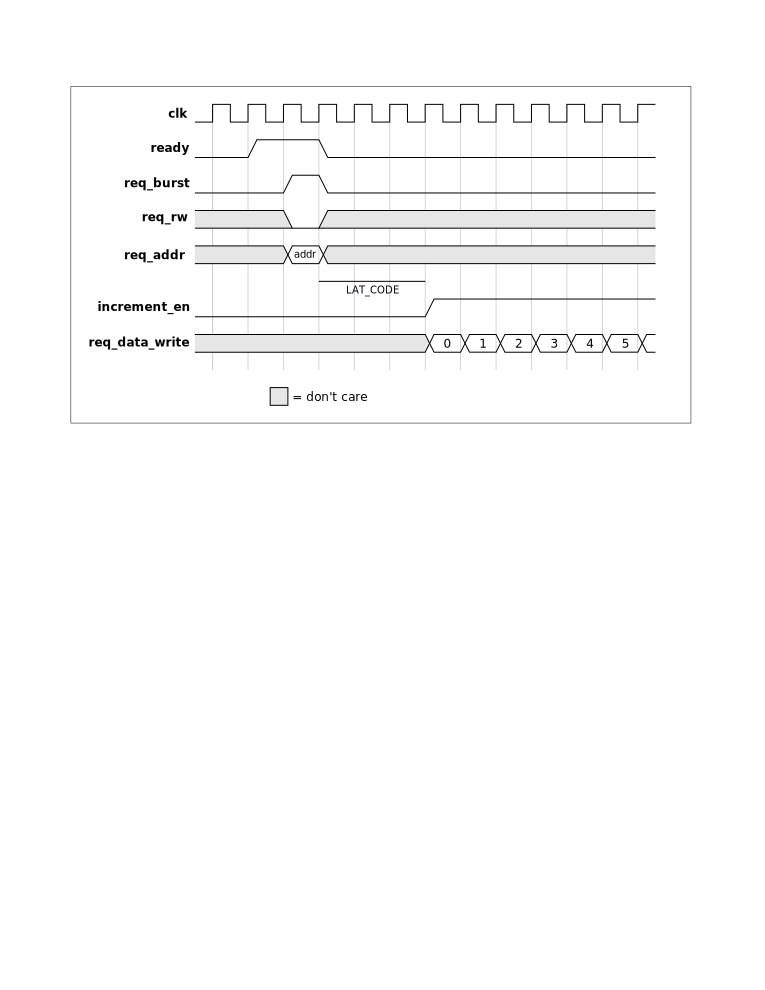
\includegraphics[width=6in]{write_start.pdf}
	\caption{Write sequence timing diagram}
\end{figure}

\begin{figure}[h]
	\includegraphics[width=6in]{write_end.pdf}
	\caption{End of write sequence}
\end{figure}

During write operations, \texttt{write\_increment\_en} is asserted to indicate that data is being latched into the IO block; this signal is intended to control a FIFO or register file pointer, and eliminates the need for the host to keep track of burst lengths. After all data has been latched into the external RAM, \texttt{done} is asserted for exactly one clock cycle.

\pagebreak

\begin{figure}
	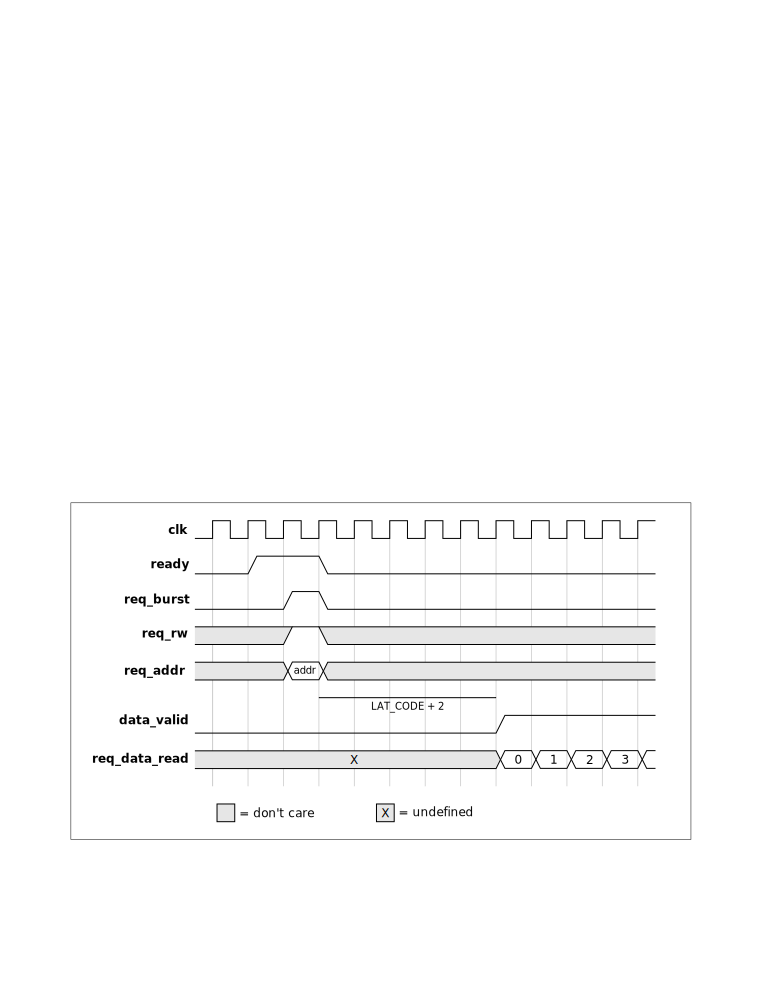
\includegraphics[width=6in]{read_start.pdf}
	\caption{Read sequence timing diagram}
\end{figure}

\begin{figure}[h]
	\includegraphics[width=6in]{read_end.pdf}
	\caption{End of read sequence}
\end{figure}

During read operations, \texttt{read\_data\_valid} is asserted to indicate that valid data has been latched in the IO block and should be read by the host.  Analogous to \texttt{increment\_en}, \texttt{read\_data\_valid} is intended to be useful in driving data into a FIFO or register file. The \texttt{done} flag is asserted for one clock cycle at the end of a read operation.

\pagebreak

\section{Implementation}

Internal FPGA signals are prone to glitches, so all outputs are registered in the IO block.  The external RAM clock is generated by a double data rate register (DDR2 primitive), and is active only when a transfer is in progress. During read operations the external RAM clock is in-phase with the system clock and during write operations it is inverted, but all connections to the host circuit are synchronous with the system clock. The address valid signal (\texttt{micronADV}) is also generated by a DDR register, to enable it to bracket the clock in both read and write modes.

\vspace{\baselineskip}

\begin{figure}[hb]
	\centering
	\includegraphics[scale=0.8]{simple_state_diagram.pdf}
	\captionsetup{singlelinecheck=on, skip=5pt}
	\caption{Simplified state diagram}
\end{figure}

\begin{figure}
	\includegraphics[width=6in]{detailed_block_diagram.pdf}
	\caption{Detailed block diagram}
\end{figure}



\end{document}